%!TEX program = xelatex
\documentclass[color=green,mathpazo,titlestyle=hang]{elegantbook}

\author{袁勇}
\email{yongyuanstu@gmail.com}
\zhtitle{基于内容的图像检索}
\zhend{实用手册}
\entitle{Practical Content-based Image Retrieval}
\enend{Handbook}
\version{2.00}
\myquote{一份以示例为驱动介绍图像处理和计算机视觉指南书}
\logo{logo.pdf}
\cover{cover.pdf}

%green color
   \definecolor{main1}{RGB}{0,120,2}
   \definecolor{seco1}{RGB}{230,90,7}
   \definecolor{thid1}{RGB}{0,160,152}
%cyan color
   \definecolor{main2}{RGB}{0,175,152}
   \definecolor{seco2}{RGB}{239,126,30}
   \definecolor{thid2}{RGB}{120,8,13}
%blue color
   \definecolor{main3}{RGB}{20,50,104}
   \definecolor{seco3}{RGB}{180,50,131}
   \definecolor{thid3}{RGB}{7,127,128}

\usepackage{makecell}
\usepackage{lipsum}
\usepackage{texnames}
\usepackage{url}

%定义python语法高亮%
%开始%
\usepackage{listings}
\usepackage{color}

\definecolor{mygreen}{rgb}{0,0.6,0}
\definecolor{mygray}{rgb}{0.5,0.5,0.5}
\definecolor{mymauve}{rgb}{0.58,0,0.82}

\lstset{ %
  numbers=left,                    %设置显示行号在左边
  frame=topline,                   %让代码周围显示边框
  backgroundcolor=\color{white},   % choose the background color
  basicstyle=\footnotesize,        % size of fonts used for the code
  breaklines=true,                 % automatic line breaking only at whitespace
  captionpos=b,                    % sets the caption-position to bottom
  commentstyle=\color{mygreen},    % comment style
  escapeinside={\%*}{*)},          % if you want to add LaTeX within your code
  keywordstyle=\color{blue},       % keyword style
  stringstyle=\color{mymauve},     % string literal style
}
%结束%


\begin{document}
\maketitle
\tableofcontents
\mainmatter

\chapter{简介}

计算机视觉的最终目标是要理解图像中的所展现的内容。对于人类而言,理解图像中的内容是极其容易的,但是对计算机而言,该任务却困难重重。

那为什么还要不辞劳苦地去学习计算机视觉呢?

因为图像无处不在!

无论是在你的智能手机上的个人照片,还是Facebook上的公共照片,亦或是YouTube上的视频,相比于过去我们有了更多的图像——并且我们需要方法来对这些图像的内容进行分析、分类,量化。

比如,你最近是否在Facebook上对你自己的或你朋友的照片加过标记?Facebook是怎样知道一幅图像中人脸的位置在哪里的?

Facebook已经在他们的网站上实现了人脸识别算法,那意味着他们不仅可以在一幅图像中找到人脸,而且他们还可以辨别出这张人脸是谁的。人脸识别技术是计算机视觉在真实世界里的一个应用。

在计算机视觉中还有没有其他类型的有用的应用呢?

当然有,我们可以利用公共图像资源库如Flickr创建我们的三维世界表示。我们可以下载由市民用他们的智能手机和照相机拍摄的成千上万的曼哈顿照片,然后对它们进行分析,并对它们进行组织来构建曼哈顿城市的三维表示,我们还可以通过我们的计算机进行该城市的可视化导航。这听起来是不是很酷?

计算机视觉另一个很火的应用是监控。

虽然监控往往有各种各样的负面含义,但是监控类型还是各有差异的。其中一类监控涉及到视频安全分析,比如抢劫后寻找可能的犯罪嫌疑人。

不过还有另一类型的在零售商店的监控。百货公司可以使用校准后的照相机来跟踪你怎么走过他们的商店,并且在哪些货架子你停下了。

你上一次去最喜欢的服装店时,你有没有在一件春天的最新潮流的牛仔裤前顿足?你在看那条牛仔裤时看了多久?你在看这些牛仔裤时的面部表情是怎样的?你有没有挑出来一条在试衣间里试穿它?所有这些类型的问题计算机视觉监控系统是能够回答的。

计算机视觉还可以应用于医学领域。一年前,我咨询了美国国家癌症研究所,该研究所研发出来了为发现癌症危险因素而能对乳腺癌组织图像进行自动分析。通常,类似这样的任务需要一个多年训练有素的病理学家—并且这将是非常耗时的!

我们的研究证明了计算机视觉可以应用于这些图像,并且能够自动的分析、量化这些细胞结构—没有人工交互!现在,我们分析乳腺组织学图像为癌症的危险因素比以往要快得多了。

当然,计算机视觉还可以用于其他的医学领域,可以用计算机视觉算法分析X-射线,MRI扫描图像以及细胞结构。

你可能听说过的最成功的计算机视觉的成功故事是X-Box 360 Kinect。Kinect用立体相机来理解图像的深度,使得它能够分辨出人类的姿势,当然,这必须得借助一些机器学习的东西。

上面列举的计算机视觉应用并不止于此。

现在计算机视觉在你生活的许多领域盛行,不管你有没有意识到它。我们用计算机视觉算法来分析电影,足球赛,手势识别(手语),车牌(比如你开车开得很快),医学,手术,军事,零售。

我们甚至可以将计算机视觉用于航天。

\chapter{Python及需要的安装包}

要探索计算机视觉世界,首先我们需要安装一些安装包。作为探索计算机视觉之旅的起始,要安装这些安装包特别是OpenCV是非常冗余乏味的,它依赖于你所使用的操作系统。我已经试着将这些安装说明简化成了一份简短的使用指南,不过,正如你所了解的,锁着项目、网站的改变,这些安装说明是会变化的!如果你在安装中遇到了问题,确保查看安装包的网站以获得最新安装说明。

我强力推荐你要么用easy\_install或pip来管理你那些安装包。它会使你的生活变得更简单!

最后,如果你不想自己逐一安装这些安装包的话,我已经预先安装好后所有需要的安装包,并把它们放在一个Ubuntu的虚拟机里。使用该虚拟机可以使你跳过那些繁琐的安装包的安装,直接进入本书的实例中,而不必理会这些安装包的管理、安装说明以及编译错误。

要想获得更多这个预先配置好的虚拟机,可以前往\url{http://www.pyimagesearch.com/practical-python-opencv/}查看详细信息。

现在,让我们来安装这些安装包!

\section{NumPy和SciPy}

NumPy是一个用于Python编程语言的库,它对大型多维数组提供支持。为什么NumPy很重要呢?原因是使用NumPy,我们可以将图像表示为一个多维数组。将图像表示为NumPy数组,不仅易于计算和资源得以有效利用,而且一些其他的图像处理操作和机器学习库也是用NumPy数组来表示的。此外,使用NumPy内置的高水准数学函数,我们能在一幅图像上做快速数值分析。

与NumPy形影不离的是SciPy。SciPy为科学和技术计算提供了更多的支持。

\subsection{Windows}

到目前为止,在你的Windows系统上安装NumPy和SciPy最简单的方式是\url{http://www.scipy.org/install.html}下载并安装二进制分发包。

\subsection{OSX}

如果你运行的是OSX 10.7.0(Lion)或更高版本,NumPy和SciPy已经预先安装好了。

不过,我喜欢安装ScipySuperpack。它包含了最新版的NumPy、SciPy、Matplotlib和其他非常有用的安装包,比如ipython、pandas和scikit-learn。所有的这些安装包是值得安装的,并且如果你在\url{www.PyImageSearch.com}上阅读我的博客,你会发现这些安装包我用得非常的频繁。

\subsection{Linux}

很多Linux发行版,比如Ubuntu,都预先安装有NumPy并且已经是配置好了的。

如果你想要最新版的NumPy和SciPy,你可以从源代码进行编译,不过最简单的方法还是用一个包管理器,比如在Ubuntu上用apt-get。

\section{Matplotlib}

用一句简洁的话概括,matplotlib是一个绘图库。如果你以前用过MATLAB,在matplotlib环境里你很可能会觉得非常的舒适。在分析图像的时候,我们会用到它。不管是画图像直方图还是只是简单地查看图像本身,matplotlib是一个非常有用的工具,你值得将它纳入到你的工具箱中。

\subsection{全平台}

Matplotlib可以在\url{http://matplotlib.org/}上下载。如果你已经安装了ScipySuperpack,那么Matplotlib就已经在你的计算机上安装了。你也可以通过easy\_install或pip来安装它。

此外,在matplotlib官网上还提供了Windows的二进制安装文件。

\section{OpenCV}

如果说NumPy的主要目标是用于有效地表示大型多维数组,那么,OpenCV的主要目标便是实时处理图像。该库从1999年发布以来,已随处可见,直到在2009年发布的第2版中我们才看到了它对NumPy的支持。OpenCV这个库本身是用C/C++写的,但在运行该安装包时它提供了Python的绑定。OpenCV是我手下最喜欢的计算机视觉库,在本书中,我们会经常使用它。

OpenCV的安装是常常会变化的。由于这个库是用C/C++写的,所以在编译的时候需要特别的注意,并要确保预先要安装的东西都已安装。由于OpenCV的最新安装说明是经常会改变的,所以在安装OpenCV时要确保自己去查看OpenCV的网站\url{http://opencv.org/}。

\subsection{Windows和linux}

OpenCV文档提供了在Windows和Linux用二进制版本安装OpenCV非常棒的教程,你可以在这里看到它的安装说明\url{http://docs.opencv.org/doc/tutorials/introduction/table_of_content_introduction/table_of_content_introduction.html#table-of-content-introduction}。

\subsection{OSX}

过去数年,在OSX上安装OpenCV是一件很痛苦的事,幸运的是现在它的安装已变得越来越简单。你需要安装cmake来构建并编译该OpenCV库,你可以从这里下载cmake\href{http://www.cmake.org/cmake/help/install.html}{http://www.cmake.org/cmake/help/install.html}。

安装cmake后,你就可以从SourceForge资源库检查源代码并进行编译。一般情况下,我发觉Guilherme Defreitas关于怎样在OSX上安装OpenCV的说明是非常棒的,并且为OpenCV的学习给出了一个很好的开始。

你可以在这里找到他的说明:\href{http://www.guidefreitas.com/installing-opencv-2-4-2-on-mac-osx-mountain-lionwith-python-support}{http://www.guidefreitas.com/installing-opencv-2-4-2-on-mac-osx-mountain-lionwith-python-support}。

\section{Mahotas}

如OpenCV一样,Mahotas也依赖于NumPy数组。很多在Mahotas中实现的函数都可以在OpenCV中找到,不过在某些情况下,Mahotas接口比OpenCV接口更容易使用,我们将用Mahotas作为OpenCV的补充。

\subsection{全平台}

在不同的平台上安装Mahotas是极其容易的。假设你已经安装了MumPy和SciPy,那么你所有需要做的只是运行pip install mahotas或easy install mahotas。

既然我们已经安装了所有我们需要的安装包,现在就让我们开始探索计算机视觉世界之旅吧!

\subsection{跳过安装}

正如我在前面提到过,安装这些安装包是费时且繁琐的。如果你想跳过上面那些安装过程而直接进入图像处理和计算机视觉世界,我已经打包好了一个预先配置好了的Ubuntu虚拟机,该虚拟机安装好了上面提到的所有安装包。

如果你对该虚拟机感兴趣并且想要下载它的话(它能够节省你很多时间并避免很多麻烦),你可以到这里下载\href{http://www.pyimagesearch.com/practicalpython-opencv/}{http://www.pyimagesearch.com/practicalpython-opencv/}。

\chapter{载入、显示及保存}

这本书的初衷是成为一本实用手册,用于指引怎样用Python和OpenCV来开始计算机视觉编程。本着这样一条信念,那就让我们不要浪费任何时间了。拿起你的键盘开始写些简单的代码,用于从磁盘载入一幅图像,在屏幕上显示它,并将它用不同的格式写入一个文件。在执行该代码的时候,我们的Python脚本应该可以在屏幕上显示我们载入的图像,正如图3.1所示。

首先,我们创建一个名为load\_display\_save.py来包含我们的代码,现在我们可以开始写代码了:

列表 3.1: load\_display\_save.py

\begin{lstlisting}[language=python]
import argparse
import cv2

ap = argparse.ArgumentParser()
ap.add_argument("-i", "--image", required = True,
	help = "Path to the image")
args = vars(ap.parse_args())
\end{lstlisting}

我们要做的第一件事是导入在这个例子中我们需要的包。我们用了argparse来解析我们的命令行参数。然后,导入cv2 - 这里cv2就是我们的OpenCV库,它包含了我们需要的图像处理函数。

\begin{figure}[!hbtp]
\centering  %使图片居中显示
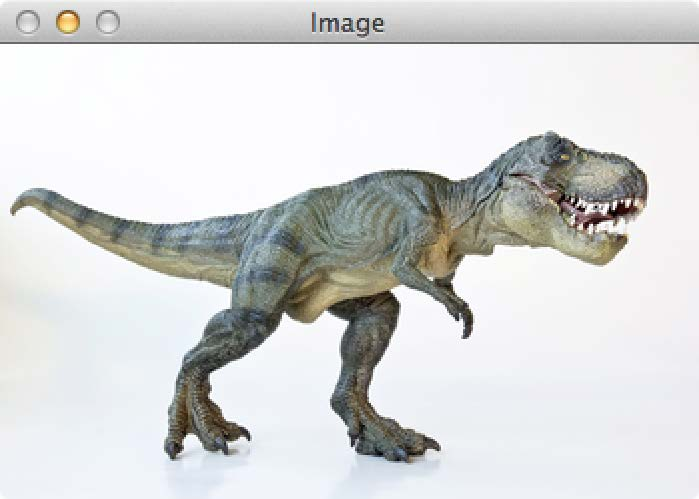
\includegraphics[width=0.8\textwidth]{figure-31.jpg}
\caption{载入并在屏幕上显示一幅霸王龙图像的例子\label{figur:Tyrannosaurus-Rex}}
\end{figure}

上面代码\textbf{第4-7行}用于解析命令行参数。这里我们需要的唯一一个参数是--image:磁盘上图像所在的路径。最后,我们解析这些参数,并在它们保存在一个字典中。

列表 3.2: load\_display\_save.py

\begin{lstlisting}[language=python]
image = cv2.imread(args["image"])
print "width: %d pixels" % (image.shape[1])
print "height: %d pixels" % (image.shape[0])
print "channels: %d" % (image.shape[2])

cv2.imshow("Image", image)
cv2.waitKey(0)
\end{lstlisting}

既然我们有了图像所在的路径,在\textbf{第8行}我们就可以用cv2.imread函数从磁盘载入该图像。cv2.imread函数返回一个NumPy数组,用于表示一幅图像。

\textbf{第9-11行}检查图像的维数。由于图像是用NumPy数组来表示的,我们可以用shape属性来检查该图像的宽、高,以及颜色通道数。

最后,\textbf{第13行}和\textbf{第14行}用于在屏幕上显示实际载入的图像。cv2.imshow的第一个参数是一个字符串,是窗口的“名字”;第二个参数是我们在\textbf{第8行}从磁盘载入的图像。最后调用了cv2.WaitKey函数来暂停运行的脚本,直到我们在键盘上按下一个键。用参数“0”表示按下任意一个键就会释放暂停。

最后,我们将该幅图像以JPG的格式写入文件中:

列表 3.3: load\_display\_save.py

\begin{lstlisting}[language=python]
cv2.imwrite("newimage.jpg", image)
\end{lstlisting}

要运行上面的脚本并显示出图片,我们只需要打开终端窗口,并执行下面的命令:

列表 3.4: load\_display\_save.py

\begin{lstlisting}[language=bash]
$ python load_display_save.py --image ../images/trex.png
\end{lstlisting}

如果不错什么问题的话,你应该可以在你的屏幕上看到\textbf{图3.1}中的霸王龙。要终止脚本的执行的话,只需要在图像窗口上单击,并按下任意键。

检查上面脚本的输出结果,你应该可以看到图片的一些基本信息。你会看到对于那张霸王龙图片,它的宽是350个像素,高是228个像素,以及3个颜色通道(R、G、B三个颜色通道)。用一个NumPy数组表示的话,该数组大小为(350,228,3)。

当我们在写矩阵时,通常我们会将它们写成这种形式:\# 行 $\times$ \#列——但对于NumPy,便不是这样的了。NumPy通常会先给出列数,然后才是行数。这点,你要牢牢记住。

最后,注意文件夹里的内容。你会看到有一个新文件在那儿:newimage.jpg。OpenCV会自动地为我们将PNG格式的图片转换为JPG格式图片!所以在图像格式间进行转换时我们并不需要费什么劲。

下一章,我们将探索怎样在一幅图像上获取像素值并对像素值进行操作。

\chapter{图像基础}

在这一章中,我们将{\color{red}{审查图像的积木}}——像素。我们将详细的讨论什么是像素,以及像素是怎样形成一幅图像的,并且怎么在OpenCV里对这些像素进行操作。

每幅图像由像素集组成。像素是一幅图像的{\color{red}{原材料,积木}}。它是图像的最小单元。

一般情况下,像素通常采用两种方式进行表示:灰度和彩色。在灰度图像中,每一个像素的像素值在0到255之间,“0”代表“黑色”,“1”表示“白色”。

\chapter{特征编码}

在这一章中,我们将{\color{red}{审查图像的积木}}——像素。我们将详细的讨论什么是像素,以及像素是怎样形成一幅图像的,并且怎么在OpenCV里对这些像素进行操作。

\subsection{Fisher Vector}

每幅图像由像素集组成。像素是一幅图像的{\color{red}{原材料,积木}}。它是图像的最小单元。

一般情况下,像素通常采用两种方式进行表示:灰度和彩色。在灰度图像中,每一个像素的像素值在0到255之间,“0”代表“黑色”,“1”表示“白色”。

\subsection{VLAD}

每幅图像由像素集组成。像素是一幅图像的{\color{red}{原材料,积木}}。它是图像的最小单元。

一般情况下,像素通常采用两种方式进行表示:灰度和彩色。在灰度图像中,每一个像素的像素值在0到255之间,“0”代表“黑色”,“1”表示“白色”。

\bibliographystyle{ieeetr}
\bibliography{reference}
\addcontentsline{toc}{chapter}{参考文献}

\end{document}
